\documentclass[10pt,letterpaper]{article}
\usepackage[utf8]{inputenc}
\usepackage{amsmath}
\DeclareMathOperator{\sign}{sgn}
\usepackage{amsfonts}
\usepackage{amssymb}
\usepackage[margin=0.5in]{geometry}
\usepackage{graphicx}
\usepackage{sidecap}
\usepackage{float}

\usepackage[font=small,labelfont=bf]{caption}


\title{\vspace{-4ex}Neural Networks\vspace{-3.5ex}}
\begin{document}
\newgeometry{top=0.75in,left=0.75in,right=0.75in,bottom=1in}
\maketitle
\vspace{-0.5em}
\begin{abstract}
In this short paper we will discuss the fundamentals of neural networks and their implementation in detail. We will give a general overview of how neural networks work, discuss calculation of the gradient and implementation of back-propagation, and test our results on some sample data (classifying toys into three subclasses) and a real dataset (the MNIST data for classifying pixels of handwritten letters). We will discuss our findings and analyze them in the context of choosing parameters and learning for our neural network.
\end{abstract}
\section{Implementation Details}
Neural networks have been around for at least a few decades, but only recently have them become popular as a method for learning parameters that can correctly translate an input into an output. This is because of increased computational power, a greater availability of training data, as well as the fact that more complex models, like deep neural nets, are actually easy to train - the same back-propagation that works to update normal neural networks works just as well for multiple hidden layers.
\begin{figure}[!htb]
\centering
\minipage{0.5\textwidth}
  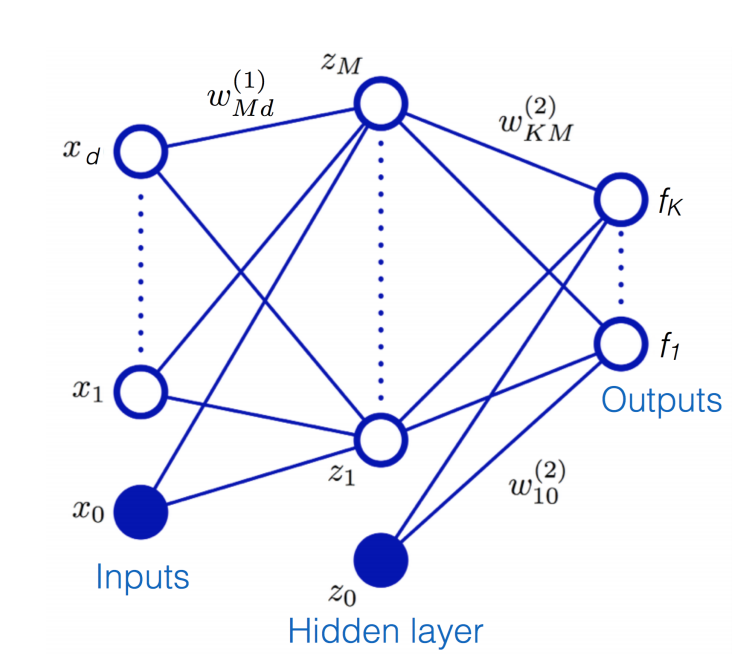
\includegraphics[width=\linewidth]{figures/neural.png}
  \caption{1-hidden layer neural networ taken from Bishop}\label{fig:neural}
\endminipage\hfill
\end{figure}
Figure 1 shows a basic neural network. The $x$ on the left is the input, with each of the $d$ dimensions acting as a separate node. These are then multiplied by the appropriate weights, added to a \textit{bias} (representing $x_0$ here), in order to obtain the \textit{activations} $a_j$ for $1\le j\le M$. These activations are then put through some non-linear map, in this case the sigmoid function, to obtain the values at the first hidden layer $z_j$. Mathematically, this looks like:
$$a_j^{(1)} = \sum_{i=1}^d w_{ji}^{(1)}x_i+w_{j0}^{(1)}$$
$$z_j = g(a_j^{(1)}) = \frac{1}{1 + e^{-a_j^{(1)}}}$$

To arrive at a simple one-hidden-layer neural network, we do this all over again, using our previous hidden layer node values (our $z_j$) instead of our inputs $x_i$ as the inputs to the second layer. The equations for this layer are analogous:
$$a_k^{(2)} = \sum_{j=1}^d w_{kj}^{(2)}x_j+w_{k0}^{(1)}$$
$$f_k = g(a_k^{(2)}) = \frac{1}{1 + e^{-a_k^{(2)}}}$$

In this paper, we will consider a loss function in the form of a negative log likelihood, taking the form:
$$\ell(w) = \frac{1}{N}\sum_{i=1}^N\sum_{k=1}^K\left[-y_k^{(i)}\log(h_k(x^{(i)},w))-(1-y_k^{(i)})\log(1-h_k(x^{(i)},w))\right]$$
where $f_k=h_k$ and $y_k$ is a $K$-dimensional one-hot vector with all 0 values except for a 1 in the $k$th dimension. If we optimize this directly, however, we will often overfit to the training data (of which we have $n$ samples from $x^{(1)}$ to $x^{(n)}$ - we distinguish these from $x_i$, which are the features of one particular sample that we will consider at a time). Thus, we add a regularization term on the weights $w^{(1)}$ and $w^{(2)}$, so that we try to minimize:
$$J(w) = \ell(w)+\lambda(||w^{(1)}||_F^2+||w^{(2)}||_F^2)$$
To do this, we can use our gradient descent methods from previous examinations of regression and classification; in this scenario, we want $\nabla_{w_1}J(w)$ and $\nabla_{w_2}J(w)$, which we can calculate analytically. First we compute:
$$\frac{\partial J(w)}{\partial h_k(x^{(i)},w)}=-\frac{y_k^{(i)}}{h_k(x^{(i)},w)}+\frac{1-y_k^{(i)}}{1-h_k(x^{(i)},w)}+2\lambda(||w^{(1)}||+||w^{(2)}||)$$
From the lecture notes, we have an expression for $\nabla_{w^{(2)}_k}J(w)$:
\begin{align*}
\nabla_{w^{(2)}_k}J(w)&=\frac{\partial J(w)}{\partial h_k(x^{(i)},w)}(\tilde{g}'(a_k^{(2)}))\textbf{z}\\
&=\frac{\partial J(w)}{\partial h_k(x^{(i)},w)}\frac{a_k^{(2)}}{e^{a_k^{(2)}}+1}\textbf{z}
\end{align*}
and this can be implemented with gradient descent and back-propagation to minimize the error. Similarly, we can calculate $\nabla_{w_1}J(w)$. First we let
$$\frac{\partial J(w)}{\partial a_k^{(2)}}=\frac{\partial J(w)}{\partial h_k(x^{(i)},w)}\frac{a_k^{(2)}}{e^{a_k^{(2)}}+1}=\delta_k^{(2)}$$
so that
$$\nabla_{w^{(2)}_k}J(w)=\delta_k^{(2)}\textbf{z}$$
Then, if we keep applying the chain rule like we did previously for $\nabla_{w^{(2)}_k}J(w)$, we'll get:
$$\nabla_{w^{(1)}_j}J(w)=\left(\frac{\partial J(w)}{\partial a_j^{(1)}}\right)\left(\nabla_{w^{(1)}_k}a_j^{(1)}\right)$$
where
\begin{align*}
\frac{\partial J(w)}{\partial a_j^{(1)}}&=\sum_{k=1}^K\left(\frac{\partial J(w)}{\partial a_k^{(2)}}\right)\left(\frac{\partial a_k^{(2)}}{\partial a_j^{(1)}}\right)\\
&=\sum_{k=1}^K\delta_k^{(2)}\cdot w_{kj}^{(2)}\cdot g'(a_j^{(1)})\\
&=\sum_{k=1}^K\delta_k^{(2)}\cdot w_{kj}^{(2)}\cdot \frac{a_j^{(1)}}{e^{a_j^{(1)}}+1} = \delta_j^{(1)}
\end{align*}
When we combine everything, we now have
$$\nabla_{w^{(1)}_j}J(w)=\delta_j^{(1)}\textbf{x}$$.

We can now use these formulas to implement our gradient descent or stochastic gradient descent based on our data and our choosing.

\section{Applications}
First, we can investigate the use of our neural network in classifying toy data. We use cross-validation to help us optimize the number of hidden nodes, and we also test both batch and stochastic gradient descent to help us find the optimal parameters. We can initialize our parameters with $w^{(1)}_{ij}$ and $w^{(2)}_{jk}$ equal to 1 for all $i,j,k$ and $M=10$. $d$ and $K$ are determined by the input vector and the number of ``groups'' we wish to classify into.
\end{document}







